\documentclass[a4paper,11pt]{article}
\usepackage[utf8]{inputenc}
\usepackage[spanish]{babel}
\usepackage[hmargin=3cm, vmargin=3cm]{geometry}
\usepackage{graphicx}
\usepackage{amssymb}
\usepackage{amsmath}
\usepackage{enumitem}
\usepackage{subcaption}
\usepackage{fancyhdr}
\usepackage{titlesec}


\titleformat{\section}
  {\bf}{Problema \thesection.}{0.5em}{}


%%%%%%%%%%%%%%%%%%%%%%%%%%%%%%%%%%%%%%%%%%%%%%%%%%%%%%%%%%%%%%%%%%%%%%%%%%%%%%

\begin{document}


% Fancy Header
% ------------
\pagestyle{fancy}
%~ \renewcommand{\headrulewidth}{0pt}
\lhead{\small Veronica Gargiulo}
\chead{\small \the\year}
\rhead{\small Santiago Soler}



% Title
% -----
\thispagestyle{plain}
\begin{center}
    \textbf{\large
        Mecánica Estadística \\
        Práctica 1 - Colectivo Microcanónico
    }
\end{center}
\vspace{-1.5em}



% Excersises
% ----------
\section{}

 Suponiendo que la entropía $S$ y la cantidad de microestados 
$\Omega$ de un sistema físico están relacionadas por una función 
arbitraria $f$ tal que:
~
$$ S = f(\Omega), $$
~
\noindent demuestre que el carácter extensivo de $S$ y el multiplicativo de 
$\Omega$ necesariamente requieren que $f$ sea de la forma:
~
$$ S = k \ln \Omega $$



\section{Aproximación de Stirling}

Mostrar que $\ln N! = \sum_{n=0}^N \ln n$.
Aproximando esta suma por una integral, obtener la aproximación de 
Stirling:
~
$$ \ln N! \simeq N \ln N - N $$



\section{Defectos Puntuales en Redes Cristalinas}

Los átomos que conforman un sólido cristalino se encuentran 
dispuestos en los vértices de una red regular (conocida como red 
cristalina) de manera compacta (Fig. \ref{fig:nacl}).
Sin embargo, a temperaturas distintas de cero, las redes cristalinas 
puede presentar defectos que rompen esa regularidad, los cuales se 
clasifican según su geometría: defectos puntuales, lineales o 
tridimensionales.

Dentro de los defectos puntuales podemos hallar las \emph{vacantes de 
Schottky}, las cuales consisten en que algunos átomos abandonen su 
posición en la red (dejando una vacante o vacío en su lugar) y migren 
hacia la superficie (Fig. \ref{fig:schottky}); y los \emph{intersticios 
de Frenkel}, en cuyo caso los átomos migran a posiciones intersticiales 
de la red (Fig. \ref{fig:frenkel}).


\vspace{1em}
\textbf{Vacantes de Schottky}
\vspace{0.5em}

Consideremos un cristal aislado ($E = $ cte) compuesto por $N$ átomos 
que presenta $n$ vacantes de Schottky.
Si suponemos que cada defecto conlleva un coste energético $\epsilon$:


\begin{figure}[b]
    \centering
    \begin{subfigure}[b]{0.3\textwidth}
        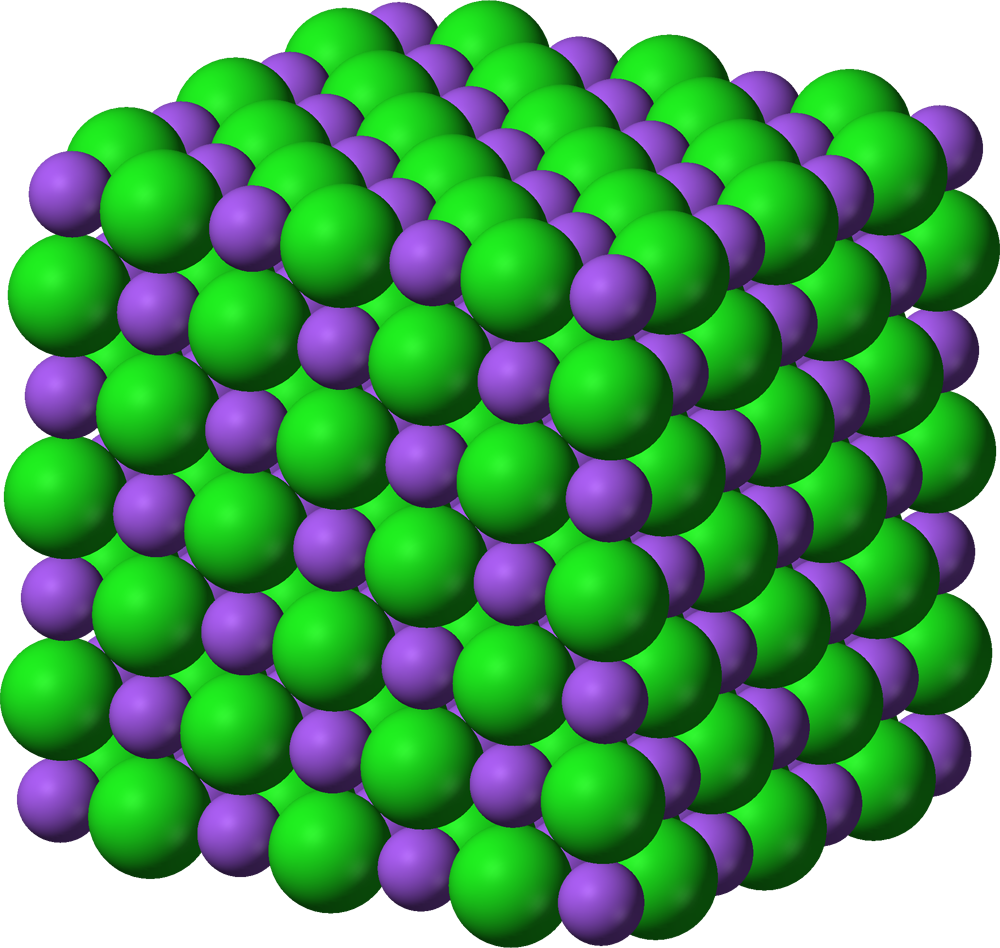
\includegraphics[width=\textwidth]{figs/NaCl.png}
        \caption{Red Cristalina de NaCl}
        \label{fig:nacl}
    \end{subfigure}
    ~
    \begin{subfigure}[b]{0.3\textwidth}
        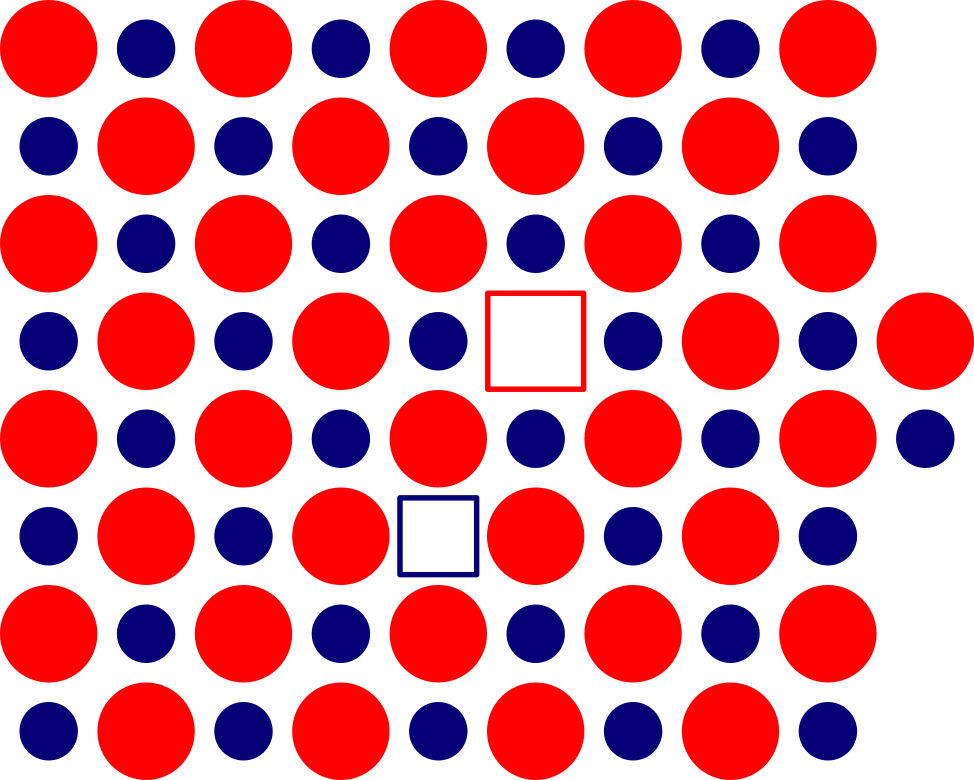
\includegraphics[width=\textwidth]{figs/schottky.png}
        \caption{Vacantes de Schottky}
        \label{fig:schottky}
    \end{subfigure}
    ~
    \begin{subfigure}[b]{0.27\textwidth}
        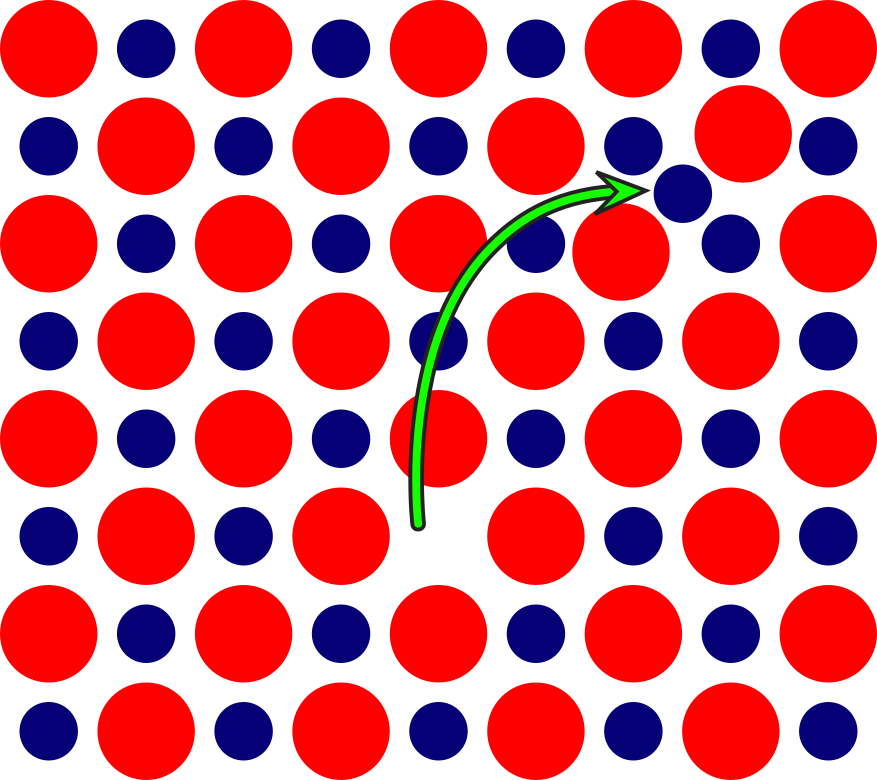
\includegraphics[width=\textwidth]{figs/frenkel.png}
        \caption{Intersticios de Frenkel}
        \label{fig:frenkel}
    \end{subfigure}
    \caption{Redes cristalinas y defectos puntuales}
\end{figure}


\begin{enumerate}[label=(\alph*),
                  leftmargin=2\parindent,
                  rightmargin=2\parindent]

    \item{\label{item:schottky-microestados}
          Calcular la cantidad de microestados $\Omega(E, N)$ en 
          función de la cantidad de defectos $n$.
          }

    \item{\label{item:schottky-entropia}
          Determinar la entropía del cristal.}
    
    \item{\label{item:schottky-defectos}
          Obtener una expresión para la cantidad de defectos en 
          función de la temperatura del cristal.
          Calcular la fracción de defectos puntuales si
          $\epsilon = 1 \text{eV}$ y $T = 300 \text{K}$.
          }

    {\small
    \textbf{Dato:}
    Un electronvoltio (eV) es una unidad de energía que equivale a 
    $1.602176565 \cdot 10^{-19}$ J.
    }
    
    \item{\label{item:schottky-cv}
          Calcular el calor específico del cristal y sus límites
          a $T = 0 \text{K}$ y $T \rightarrow \infty$.
          Realizar una gráfica del mismo en función de $T$.
          }

    \item{Teniendo en cuenta que la organización compacta de los átomos 
          en los vértices de la red cristalina minimiza la energía 
          interna del sistema, ¿cómo puede interpretar el hecho de que 
          la red presente defectos puntuales (a temperatura distinta de 
          cero) si cada defecto implica un costo energético?
          }

\end{enumerate}


\textbf{Intersticios de Frenkel}
\vspace{0.5em}

Responder los puntos \ref{item:schottky-microestados}, 
\ref{item:schottky-entropia} y \ref{item:schottky-defectos} del 
ejercicio anterior considerando el mismo cristal, pero que ahora 
presenta $n$ átomos situados en sitios intersticiales (solo defectos de 
Frenkel).

\vspace{0.5em}
{\small
\textbf{Ayuda:} Considere la red del cristal y una red dual (de 
instersticios) a la cual van a parar los átomos que migran. Es válido 
suponer que ambas redes poseen la misma cantidad de sitios.
}



\section{Paramagneto}

Una sustancia paramagnética es aquella que presenta magnetización 
$\mathbf{M}$ nula frente a un campo magnético externo $\mathbf{H}$ 
nulo.
Si por el contrario, el campo no es nulo, el paramagneto se imanta en 
la misma dirección que $\mathbf{H}$. Se pueden considerar dos clases de 
paramagnetismo: el regular o el de \emph{Pauli}.
El segundo se debe al gas de electrones libres de un metal, mientras 
que el primero se origina en la interacción de los momentos magnéticos 
intrínsecos de los átomos del sólido con el campo magnético externo.
En este problema analizaremos un caso sencillo del magnetismo de 
Langevin.

Supongamos un paramagneto inmerso en un campo magnético $H$ 
orientado en la dirección del eje $z$.
Consideremos que el paramagneto está compuesto por $N$ momentos 
magnéticos individuales (y no interactuantes entre sí) de manera tal 
que la proyección de cada momento magnético en el eje $z$ 
puede ser $\pm \mu_B$ ($\mu_B = e\hbar / 2m_e c = 9.273 \times 
10^{-24} \text{J/T}$ se conoce como el magnetón de Bohr).
La magnetización total del sistema estará dada por $M = m \mu_B$, donde 
$N/2 + m/2$ y $N/2 - m/2$ son las cantidades de momentos magnéticos que 
apuntan hacia arriba y hacia abajo, respectivamente.
Vamos a considerar también que el sistema ``paramagneto + campo 
magnético'' es un sistema aislado, es decir, $E = - 
\mathbf{M}\cdot\mathbf{H} = \text{cte}$.

\begin{enumerate}[label=(\alph*),
                  leftmargin=2\parindent,
                  rightmargin=2\parindent]

    \item{Encontrar una expresión analítica para el número de 
          estados microscópicos $\Omega(N, M)$ correspondientes a una 
          magnetización total M.
          }
    
    \item{\label{item:paramagneto-magnetizacion}
          Usando la relación
          $\frac{1}{T} = \left( \frac{\partial S}{\partial E} \right)_V$,
          hallar la ecuación de estado de los paramagnetos:
          $$ M = N \mu_B \tanh \left( \frac{\mu_B H}{k_B T} \right) $$.
          }
    
    \item{\label{item:paramagneto-grafica}
          Realizar una gráfica de $M$ vs $\mu_B H/k_B T$.
          ¿Qué sucede con la magnetización a altas temperaturas?
          ¿Qué sucede con la magnetización a bajas temperaturas?
          }
    
    {\small
    \textbf{Ayuda:} Cuando hablamos de bajas temperaturas nos referimos 
    a que $k_B T \ll \mu_B H$, mientras que altas temperaturas 
    significa que $k_B T \gg \mu_B H$.
    }

    \item{La Ley de Curie (obtenida experimentalmente por Pierre Curie en 1896)
          establece que la magnetización de un paramagneto es 
          directamente proporcional al campo magnético externo e 
          inversamente proporcional a la temperatura:
          $$ M \propto \frac{H}{T} $$
          Determinar el rango de validez de la Ley de Curie a partir de la
          gráfica realizada en \ref{item:paramagneto-grafica}
          (¿altas o bajas temperaturas?).\\
          Obtener la Ley de Curie a partir de un desarrollo en series 
          de Taylor de la magnetización obtenida en 
          \ref{item:paramagneto-magnetizacion}.
          }
    
    \item{Si consideramos un paramagneto compuesto por $N = 10^{24}$ 
          momentos magnéticos a $T = 300 \text{K}$ y sometido a un 
          campo magnético externo $H = 10^{-3} T$,
          ¿cuál es la energía necesaria para invertir totalmente la 
          magnetización $M$?
          }

    \item{Calcular el calor específico del paramagneto y realizar una 
          gráfica del mismo en función de $\mu_B H / k_B T$.
          ¿Cómo podemos interpretar el pico que presenta el calor específico?
          }

\end{enumerate}



\section{Sólido de Einstein}

Uno de los primeros modelos que se propusieron para describir las vibraciones 
de un sólido cristalino es el de Einstein. El mismo considera cada uno de los 
$N$ átomos del sólido vibrando alrededor de su posición de equilibrio y de 
manera independiente. Además, presupone que todos los átomos oscilan con la 
misma frecuencia $\omega$. Si consideramos a cada átomo como un oscilador 
harmónico cuántico 3D, cada uno posee niveles de energía discretos
($n = 1, 2, 3, \dots$) y por ende, la energía total del sistema ($E$) puede 
distribuirse entre los distintos osciladores en $E/\hbar\omega$ 
cuantos de energía.

\begin{enumerate}[label=(\alph*),
                  leftmargin=2\parindent,
                  rightmargin=2\parindent]

    \item{Calcular la cantidad de microestados $\Omega(E, N, V)$:\\
          $$\Omega(E, N, V) =
          \frac{(3N - 1 + E/\hbar\omega)!}{(3N - 1)! \, (E/\hbar\omega)!}$$
          }

    \item{Obtener una expresión para la energía total $E$ en función 
          de la temperatura y analizar los límites a la temperatura del 
          cero absoluto y a temperaturas altas ($T \rightarrow \infty$).
          }

    \item{Calcular el calor específico del sólido de Einstein.
          Analizar los casos de $T=0 \text{K}$ y $T \rightarrow \infty$.
          Realizar una gráfica del $C_v$ en función de $T$
          (utilizar Software como wxMaxima).
          }
\end{enumerate}

{\small
\textbf{Ayuda 1:} Los niveles de energía de un oscilador harmónico cuántico 
unidimensional vienen dados por: $E_n = (n + 1/2) \hbar \omega$.

\textbf{Ayuda 2:} Al considerar cada átomo como un oscilador 3D, podemos asumir
que el sólido de $N$ átomos es equivalente a un sistema de $3N$ osciladores
harmónicos 1D. Además, podemos realizar un corrimiento de la energía total
del sistema y de esta manera considerar nula la energía de punto cero del
oscilador.
}

\end{document}

